\documentclass[]{book}
\usepackage{lmodern}
\usepackage{amssymb,amsmath}
\usepackage{ifxetex,ifluatex}
\usepackage{fixltx2e} % provides \textsubscript
\ifnum 0\ifxetex 1\fi\ifluatex 1\fi=0 % if pdftex
  \usepackage[T1]{fontenc}
  \usepackage[utf8]{inputenc}
\else % if luatex or xelatex
  \ifxetex
    \usepackage{mathspec}
  \else
    \usepackage{fontspec}
  \fi
  \defaultfontfeatures{Ligatures=TeX,Scale=MatchLowercase}
\fi
% use upquote if available, for straight quotes in verbatim environments
\IfFileExists{upquote.sty}{\usepackage{upquote}}{}
% use microtype if available
\IfFileExists{microtype.sty}{%
\usepackage{microtype}
\UseMicrotypeSet[protrusion]{basicmath} % disable protrusion for tt fonts
}{}
\usepackage[margin=1in]{geometry}
\usepackage{hyperref}
\hypersetup{unicode=true,
            pdftitle={Data Science for the Liberal Arts},
            pdfauthor={Kevin Lanning},
            pdfborder={0 0 0},
            breaklinks=true}
\urlstyle{same}  % don't use monospace font for urls
\usepackage{natbib}
\bibliographystyle{apalike}
\usepackage{longtable,booktabs}
\usepackage{graphicx,grffile}
\makeatletter
\def\maxwidth{\ifdim\Gin@nat@width>\linewidth\linewidth\else\Gin@nat@width\fi}
\def\maxheight{\ifdim\Gin@nat@height>\textheight\textheight\else\Gin@nat@height\fi}
\makeatother
% Scale images if necessary, so that they will not overflow the page
% margins by default, and it is still possible to overwrite the defaults
% using explicit options in \includegraphics[width, height, ...]{}
\setkeys{Gin}{width=\maxwidth,height=\maxheight,keepaspectratio}
\IfFileExists{parskip.sty}{%
\usepackage{parskip}
}{% else
\setlength{\parindent}{0pt}
\setlength{\parskip}{6pt plus 2pt minus 1pt}
}
\setlength{\emergencystretch}{3em}  % prevent overfull lines
\providecommand{\tightlist}{%
  \setlength{\itemsep}{0pt}\setlength{\parskip}{0pt}}
\setcounter{secnumdepth}{5}
% Redefines (sub)paragraphs to behave more like sections
\ifx\paragraph\undefined\else
\let\oldparagraph\paragraph
\renewcommand{\paragraph}[1]{\oldparagraph{#1}\mbox{}}
\fi
\ifx\subparagraph\undefined\else
\let\oldsubparagraph\subparagraph
\renewcommand{\subparagraph}[1]{\oldsubparagraph{#1}\mbox{}}
\fi

%%% Use protect on footnotes to avoid problems with footnotes in titles
\let\rmarkdownfootnote\footnote%
\def\footnote{\protect\rmarkdownfootnote}

%%% Change title format to be more compact
\usepackage{titling}

% Create subtitle command for use in maketitle
\newcommand{\subtitle}[1]{
  \posttitle{
    \begin{center}\large#1\end{center}
    }
}

\setlength{\droptitle}{-2em}
  \title{Data Science for the Liberal Arts}
  \pretitle{\vspace{\droptitle}\centering\huge}
  \posttitle{\par}
  \author{Kevin Lanning}
  \preauthor{\centering\large\emph}
  \postauthor{\par}
  \predate{\centering\large\emph}
  \postdate{\par}
  \date{2018-02-12}

\usepackage{booktabs}

\usepackage{amsthm}
\newtheorem{theorem}{Theorem}[chapter]
\newtheorem{lemma}{Lemma}[chapter]
\theoremstyle{definition}
\newtheorem{definition}{Definition}[chapter]
\newtheorem{corollary}{Corollary}[chapter]
\newtheorem{proposition}{Proposition}[chapter]
\theoremstyle{definition}
\newtheorem{example}{Example}[chapter]
\theoremstyle{definition}
\newtheorem{exercise}{Exercise}[chapter]
\theoremstyle{remark}
\newtheorem*{remark}{Remark}
\newtheorem*{solution}{Solution}
\begin{document}
\maketitle

{
\setcounter{tocdepth}{1}
\tableofcontents
}
\part{Part I Introduction}\label{part-part-i-introduction}

This work-in-progress includes the notes for
\href{https://kevinlanning.github.io/DataSciSpring2018/}{\emph{\emph{Introduction
to Data Science}}} at the Wilkes Honors College of Florida Atlantic
University. It's written using the R package Bookdown
\citep{R-bookdown}.

\chapter{Data science for the liberal
arts}\label{data-science-for-the-liberal-arts}

Hochster, in \citet{hicks2017guide}, describes two broad types of data
scientists: Type A (Analysis) data scientists, whose skills are like
those of an applied \textbf{statistician}, and Type B (Building) data
scientists, whose skills lie in problem solving or coding, using the
skills of the \textbf{computer scientist}. Hochster's view of data
science arguably omits a critical component of the field. Data science
is driven not just by statistics and computer science, but also by
``domain expertise:''

\section{Type C data science}\label{type-c-data-science}

The iconic
\href{https://www.google.com/search?q=venn+diagram+model+of+data+science\&newwindow=1\&safe=active\&rlz=1C1CHBF_enUS762US763\&tbm=isch\&tbo=u\&source=univ\&sa=X\&ved=0ahUKEwiM_abBtY7XAhXDQCYKHdgyB58QsAQIOg\&biw=1378}{Venn
diagram model of data science} suggests what we can call a ``Type C data
science.'' It begins with ``domain expertise'' in your
\textbf{concentration} in the arts, humanities, social and/or natural
sciences, it both informs and can be informed by new methods and tools
of data analysis, and it includes such things as \textbf{communication}
(including writing and the design and display of quantitative data),
\textbf{collaboration} (making use of the tools of team science), and
\textbf{citizenship} (serving the public good, overcoming the digital
divide, furthering social justice, increasing public health, diminishing
human suffering, and making the world a more beautiful place). It's
shaped, too, by an awareness of the \textbf{creepiness} of living
increasingly in a measured, observed world.

\section{The incompleteness of the Venn
diagram}\label{the-incompleteness-of-the-venn-diagram}

The Venn diagram model is incomplete. In addition to \emph{statistics,
computing/hacking,} and \emph{domain expertise,} a number of additional
skills contribute to the success of the data scientist.

These include \emph{collaboration,} which is arguably the most
distinctive feature of contemporary scholarship in the natural and
social sciences as well as in the private sector
\citep{isaacson2014innovators}.

\emph{Communication} is central to data science because results are
inconsequential unless they are recognized, understood, and built upon;
facets of communication include oral presentations, written texts and,
too, clear data visualizations.

\emph{Reproducibility} is related to both communication and
collaboration. There has been something of a crisis in recent years in
the social and natural sciences as many results initially characterized
as ``statistically significant'' have been found not to replicate. The
reasons for this are multiple and presently contentious, but one path
towards better science includes the public sharing of methods and data,
ideally before experiments are undertaken. Reproducible methods are a
key feature of contemporary data science.

\emph{Pragmatism} refers to the relevance of work towards real-world
goals. Ideally, these pragmatic concerns take into account \emph{ethical
concerns} as well.

\section{The expertise dimension}\label{the-expertise-dimension}

Cutting across these eight facets (statistics, computing, domain
expertise, collaboration, communication, reproducibility, pragmatism,
and ethics), a second dimension can be articulated. No one of us can
excel in all eight domains, rather, we might aim towards goals ranging
from \emph{literacy} (can understand) through \emph{proficiency} (can
get by) to \emph{fluency} (can practice) to \emph{leadership} (can
create new solutions or methods).

That is, we can think of a \emph{continuum} of knowledge, skills,
interests, and goals, ranging from that which characterizes the data
\emph{consumer} to the data \emph{citizen} to the data science
\emph{contributor.} A Type C data science includes this dimension as
well.

\section{Google and the liberal arts}\label{google-and-the-liberal-arts}

Data science is at its core empirical, and all of this rhetoric would be
meaningless if not grounded in real world findings. Although it was
recently reported that
\href{https://www.washingtonpost.com/news/answer-sheet/wp/2017/12/20/the-surprising-thing-google-learned-about-its-employees-and-what-it-means-for-todays-students/?sw_bypass=true\&utm_term=.23e48235d66e}{soft
skills rather than STEM training were the most important predictors of
success among Google employees}, it's difficult to know whether these
results would generalize to a less select group. Nonetheless, there is a
clear need for individuals with well-rounded training in the liberal
arts in data science positions and, conversely, learning data science is
arguably a key part of a contemporary liberal arts education.

\section{Data sci and TMI}\label{data-sci-and-tmi}

It has been said (by whom?) that the biggest difference between
traditional stats and data science is that the former is typically
concerned with making inferences from datasets that are too
\emph{small}, while the latter is concerned with extracting a signal
from data that is or are too \emph{big}.

The struggle to extract meaning from a sea of information - of finding
needles in haystacks, of finding faint signals in a cacophany of
overstimulation - is arguably the question of the age. It is a question
we deal with as individuals on a moment-by-moment basis. It is a
challenge I face as I wade through the many things that I could include
in this class and these notes.

The \emph{primacy of editing} or selection lies at the essence of human
perception and the creation of art forms ranging from novels to film.
And it is a key challenge for the data scientist faces as well.

\section{A challenge}\label{a-challenge}

Imagine it is ten years from today. You are working in a cool job (yay).
How, ideally, would `data science' inform your professional
contributions?

More proximally (closer to today) - what are your own goals for progress
in data science, in terms of the model described above?

\chapter{Setting up your computer}\label{setting-up-your-computer}

Install R and R studio on your own laptop. If you get stuck, reach out
to others on Slack; if you don't get stuck, help your classmates.

\chapter{Pretest}\label{pretest}

Reflect on your own knowledge of data science, including the
necessary-but-not-sufficient areas of computer programming and
statistics.

You may know more than you think you do. Even if you haven't had formal
programming, you may well have experience with spreadsheets such as
Excel or Google Sheets? What does `=SUM (A1:A15)' mean? In a
spreadsheet, if `=SUM (A1:A15)' was in cell A16, and you copied this to
cell B16, what would the result be?

Statistics is, of course, relevant in a myriad of ways. Consider, for
example, the prospects for Susie, a young woman who is applying to two
Med schools. At School A, 25\% of students are accepted, and at School
B, 25\% are accepted as well.

You are Susie. Are you going to get in to at least one of these
programs? What is the probability? Does your estimate depend upon any
assumptions?

\section{A thought experiment}\label{a-thought-experiment}

Would it be possible to assign grades in a class based not just on what
students know at the end of the term, but also on how much they have
learned?

You could, in principle, do this using regression analysis. That is, you
could predict final exam scores from pretest scores, and use the
residuals - the extent to which students did better or worse than
expected - as a contributor to final exam grades.

Interestingly, there would be an unusual incentive for students on this
`pretest' to do, seemingly perversely, as poorly as possible. How might
you address this?

\chapter{Some basic tools: Slack, Markdown, Google
Docs}\label{some-basic-tools-slack-markdown-google-docs}

On Markdown, see \citet{freeman2017informatics}, Chapter 3). Some
Markdown editors include Typora, Atom, and Ghostwriter.

R markdown is a `flavor' of - wait for it - markdown. For beginning with
R markdown, consider
\href{https://idc9.github.io/stor390/notes/getting_started/getting_started.html}{Carmichael
(2017) Getting started} as well as the first chapter of
\citet{wickham2016r}.

Slack is a messaging and collaboration platform. There is a simple
markdown editor in Slack (for `posts').

You are likely to be familiar with Google Docs as well. One interesting
feature of Google Docs is that it provides some basic tools for
\emph{version control,} a critical skill in information management
particularly (but not only) for collaborative work. You can learn more
about how to see prior versions of a project in Google Docs
\href{https://sites.google.com/site/scriptsexamples/home/announcements/named-versions-new-version-history-google-docs}{here}
.

Version control can help you avoid the chaos and confusion of having a
computer full of files that look like Cham's (2012) comic:

.

Never call anything `final.doc'.

We'll be talking about the challenge of version control throughout this
text - and I am hoping that my own habits in file management can improve
as we move forward together.

\chapter{An introduction to R}\label{an-introduction-to-r}

R is a system for reproducible science, and reproducibility is essential
\citep{baumer2014r}. R is a system for Representing data in cool,
insight-facilitating ways. R is really popular, and really growing.
Learning R will make you a more attractive candidate for many graduate
programs as well as jobs in the private sector.

\subsection{\texorpdfstring{One does not `learn
R'}{One does not learn R}}\label{one-does-not-learn-r}

Unlike, say, learning to ride a bicycle, fry an egg, or drive a car with
a manual transmission, learning R is not a discrete accomplishment that
one masters and then moves on. Rather, R is an evolving, open system of
applications and tools which is so vast that there is always more that
one can achieve, new lessons that one can learn.

\subsection{What R stands for}\label{what-r-stands-for}

Historically, R grew out of S which could stand for Statistics. But what
does R stand for?

R does not stand for
`\href{https://www.urbandictionary.com/define.php?term=ARGH}{argh},'
although you may proclaim this in frustration (`arggh, why can't I get
this to work?) or, perhaps, in satisfaction ('arggh, matey, that be a
clever way of doing this').

R might stand for \emph{relatively high level.} Programming languages
can be described along a continuum from high to low level, the former
(like R) are more accessible to humans, the latter (like assembly
language) more accessible to machines. Python, Java, and C++ are all
more towards the middle of this continuum.

R stands, in part, for \emph{resources.} There are many resources,
including, for example -

\begin{itemize}
\tightlist
\item
  Online resources include the simple (and less simple) lessons of
  \href{http://swirlstats.com/}{SwirlR}, which offers the possibility of
  ``learning R in R,'' as well as
  \href{https://www.datacamp.com/home}{DataCamp}, the
  \href{https://www.coursera.org/specializations/jhu-data-science}{Data
  Science Certificate Program at Johns Hopkins,} and other MOOCs.\\
\item
  Books include \citet{peng2015r} - which includes not only videos of
  his lectures in the program at Hopkins, but also a brief list of still
  more resources - and \citet{wickham2016r}.
\item
  You'll also learn (more directly) from people, including your
  classmates, as well as the broader community of people around the
  world. There are hundreds if not thousands of people, young and old,
  who are on the road with you. As I am, just a step or two (hopefully)
  ahead.
\end{itemize}

\subsection{On R Studio and commercial vs.~open
software}\label{on-r-studio-and-commercial-vs.open-software}

R Studio is a commercial enterprise whose business model, judged from
afar, is an important one in the world of technology and open science.
Most of what R Studio offers is free (97\% according to Garrett
Grolemund in the video below). The commercial product they offer makes
sense for a relative few, but it is sufficiently lucrative to fund the
enterprise. The free product helps to drive the popularity of R studio;
this widespread use, in turn, makes it increasingly essential for
businesses to use.

This mixed free/premium model characterizes Slack as well, but while
\href{https://www.statista.com/statistics/652779/worldwide-slack-users-total-vs-paid/}{the
ratio of free to paid users of Slack is on the order of 3:1}, for R it
is, I am guessing, an order of magnitude higher than this.

The openness of R is an important feature, not just because it saves you
money, but because contributing to the world of R is an act of digital
democracy, for in contributing to the world of R we open up knowledge to
others who may lack our privileges. The corporate clients of R studio,
in essence, support the rest of us.

\subsubsection{A digression and thought
experiment}\label{a-digression-and-thought-experiment}

All contemporary cars have computers. Many of these are quite
sophisticated, allowing cars to drive themselves in increasingly
autonomous ways. But the potential of autonomous cars will not be
realized until they are connected on the 'net. Communication with other
cars, stoplights, etc. will reduce travel times, increase fuel
efficiency, and increase safety, too.

Until, that is, they are hacked.

Who should be the guardians of the net linking cars? Should this be
closed (with Ford having it's own safeguards), or public?

\subsection{A few characteristics of
R}\label{a-few-characteristics-of-r}

R includes the base plus thousands of \textbf{packages}. These packages
are customized add-ons which simplify certain tasks, such as text
analysis. But there are at least \href{}{40 different packages for this}
- where do you begin? The most recent answer, and where we will start,
is the curated list of packages which jointly comprise the tidyverse
\citep{wickham2016r}.

\citet{peng2015r} speculated that ``it would be straightforward to build
an R package for ordering pizza.'' Does one exist now?

R is an object-oriented language. At an atomic level, these include
\emph{characters, real numbers, integers, complex numbers, and logical.}
These atoms are combined into vectors, which (unless they are lists)
include objects of the same type \citep{peng2015r}. Missing values may
be characterized by NA (not available) or NaN (not a number, implying an
undefined or impossible value). Attributes of R include such things as
name, dimensions (for vectors and arrays), class (that's the atomic
thing), length, etc. Vectors can be combined into a \textbf{data frame}
(or, in a simplified form, a \emph{tibble}), which greatly facilitates
statistical analysis.

\chapter{Finding help}\label{finding-help}

To get a sense of some of the ways you can get help in R studio (and to
see how a master uses the R Studio interface), consider the following
video:

\href{https://www.rstudio.com/resources/webinars/rstudio-essentials-webinar-series-part-1/?wvideo=k8kz4e0p2v}{\includegraphics{https://embedwistia-a.akamaihd.net/deliveries/fb7bd1e692d80505e8d3212678e41f2176b39fde.jpg?image_play_button_size=2x\&image_crop_resized=960x540\&image_play_button=1\&image_play_button_color=71a5d4e0}}

{[}RStudio Essentials Webinar Series -- Programming Part 1 -- RStudio
\href{https://www.rstudio.com/resources/webinars/rstudio-essentials-webinar-series-part-1/?wvideo=k8kz4e0p2v}{https://www.rstudio.com/{]}}

For us, the key ideas in ``looking for help'' will include not just the
tools on the R Studio IDE, but also (a) using google searches wisely,
and (b) reaching out to your classmates on Slack. At the next level, the
search for help should be built around reproducible errors. There is a
\href{https://cran.r-project.org/web/packages/reprex/index.html}{package}
for this.

\chapter{Empiricism \textgreater{}
intuition}\label{empiricism-intuition}

Thoughts on the first four chapters of \citet{stephens2017everybody}.
Note that \textbf{Italicized blocks are exact quotes pulled off Kindle}

\section{Health: Internet (search) data can illuminate medical
syndromes}\label{health-internet-search-data-can-illuminate-medical-syndromes}

\subsection{Pancreatic cancer}\label{pancreatic-cancer}

\emph{Searching for back pain and then yellowing skin turned out to be a
sign of pancreatic cancer; searching for just back pain alone made it
unlikely someone had pancreatic cancer. Similarly, searching for
indigestion and then abdominal pain was evidence of pancreatic cancer,
while searching for just indigestion without abdominal pain meant a
person was unlikely to have it. \ldots{} a clear example of rigorous
data science and computers teaching us things our gut alone could never
find. This is also one case where the size of the dataset matters.
Sometimes there is insufficient experience for our unaided gut to draw
upon. It is unlikely that you---or your close friends or family
members---have seen enough cases of pancreatic cancer to tease out the
difference between indigestion followed by abdominal pain compared to
indigestion alone.}

\textbf{Intuition isn't really the problem:} For Stephens-Davidowitz,
the problem is not ``intuition,'' or what Kahneman would refer to as
Type I thinking, but ``intuition based on limited data''

\subsection{Depression}\label{depression}

Seasonal Affective Disorder (SAD) is a real thing. It's evidenced in
search data too.

\emph{In winter months, warm climates, such as that of Honolulu, Hawaii,
have 40 percent fewer depression searches than cold climates, such as
that of Chicago, Illinois. Just how significant is this effect? An
optimistic read of the effectiveness of antidepressants would find that
the most effective drugs decrease the incidence of depression by only
about 20 percent. To judge from the Google numbers, a
Chicago-to-Honolulu move would be at least twice as effective as
medication for your winter blues.}

\section{The NBA}\label{the-nba}

This is really clever in several ways. First, the question. As a social
scientist, \citet{stephens2017everybody} addresses this empirically

\subsection{Are you more likely to make it in the NBA if you grow up
poor?**}\label{are-you-more-likely-to-make-it-in-the-nba-if-you-grow-up-poor}

\subsubsection{An empirical approach}\label{an-empirical-approach}

This is arguably a little weak, in that it is indirect.

\emph{It was suggested in a paper by two economists, Roland Fryer and
Steven Levitt, that a black person's first name is an indication of his
socioeconomic background. Fryer and Levitt studied birth certificates in
California in the 1980s and found that, among African-Americans, poor,
uneducated, and single moms tend to give their kids different names than
do middle-class, educated, and married parents\ldots{}California-born
NBA players were half as likely to have unique names as the average
black male, a statistically significant difference.}

\subsubsection{\texorpdfstring{Applying decision analysis : Looking at
both types of
`errors'}{Applying decision analysis : Looking at both types of errors}}\label{applying-decision-analysis-looking-at-both-types-of-errors}

In making decisions on the basis of imperfect information - such as
\emph{should we give chemotherapy?}, \emph{should we accept this person
into our grad program?} - it's often useful to think in terms of a
fourfold table, in which cells describe two types of correct decisions
and two types of errors.

\textbf{\emph{The} miss (rough/no NBA):} \emph{Let's look at the story
of \textbf{Doug Wrenn}, one of the most talented basketball prospects in
the 1990s. His college coach, Jim Calhoun at the University of
Connecticut, who has trained future NBA all-stars, claimed Wrenn jumped
the highest of any man he had ever worked with. But Wrenn had a
challenging upbringing. He was raised by a single mother in Blood Alley,
one of the roughest neighborhoods in Seattle. In Connecticut, he
consistently clashed with those around him. He would taunt players,
question coaches, and wear loose-fitting clothes in violation of team
rules. He also had legal troubles---he stole shoes from a store and
snapped at police officers. Calhoun finally had enough and kicked him
off the team. Wrenn got a second chance at the University of Washington.
But there, too, an inability to get along with people derailed him. He
fought with his coach over playing time and shot selection and was
kicked off this team as well. Wrenn went undrafted by the NBA, bounced
around lower leagues, moved in with his mother, and was eventually
imprisoned for assault. ``My career is over,'' Wrenn told the Seattle
Times in 2009. ``My dreams, my aspirations are over. Doug Wrenn is dead.
That basketball player, that dude is dead. It's over.'' Wrenn had the
talent not just to be an NBA player, but to be a great, even a legendary
player. But he never developed the temperament to even stay on a college
team.}

\textbf{The false positive (supportive/NBA):} \emph{Perhaps if he'd had
a stable early life, he could have been the next Michael Jordan. Michael
Jordan, of course, also had an impressive vertical leap. Plus a large
ego and intense competitiveness---a personality at times that was not
unlike Wrenn's. Jordan could be a difficult kid. At the age of twelve,
he was kicked out of school for fighting. But he had at least one thing
that Wrenn lacked: a stable, middle-class upbringing. His father was an
equipment supervisor for General Electric, his mother a banker. And they
helped him navigate his career.}

\emph{In fact, Jordan's life is filled with stories of his family
guiding him away from the traps that a great, competitive talent can
fall into. After Jordan was kicked out of school, his mother responded
by taking him with her to work. He was not allowed to leave the car and
instead had to sit there in the parking lot reading books. After he was
drafted by the Chicago Bulls, his parents and siblings took turns
visiting him to make sure he avoided the temptations that come with fame
and money. Jordan's career did not end like Wrenn's, with a little-read
quote in the Seattle Times. It ended with a speech upon induction into
the Basketball Hall of Fame that was watched by millions of people. In
his speech, Jordan said he tried to stay ``focused on the good things
about life---you know how people perceive you, how you respect them
.~.~. how you are perceived publicly. Take a pause and think about the
things that you do. And that all came from my parents.'' The data tells
us Jordan is absolutely right to thank his middle-class, married
parents. The data tells us that in worse-off families, in worse-off
communities, there are NBA-level talents who are not in the NBA. These
men had the genes, had the ambition, but never developed the temperament
to become basketball superstars. And no---whatever we might
intuit---being in circumstances so desperate that basketball seems ``a
matter of life or death'' does not help. Stories like that of Doug Wrenn
can help illustrate this. And data proves it.}

\textbf{The hit (rough/NBA)} \emph{In June 2013, \textbf{LeBron James}
was interviewed on television after winning his second NBA championship.
(He has since won a third.) ``I'm LeBron James,'' he announced. ``From
Akron, Ohio. From the inner city. I am not even supposed to be here.''
Twitter and other social networks erupted with criticism. How could such
a supremely gifted person, identified from an absurdly young age as the
future of basketball, claim to be an underdog? In fact, anyone from a
difficult environment, no matter his athletic prowess, has the odds
stacked against him. James's accomplishments, in other words, are even
more exceptional than they appear to be at first. Data proves that,
too.}

\textbf{The correct rejection (supportive/no NBA)} Think about this
fourth cell. What or who would define it? How would you statistically
summarize results from such a table?

\subsubsection{The power of brute force facts: The effect of
height}\label{the-power-of-brute-force-facts-the-effect-of-height}

\emph{How much does height matter? NBA players sometimes fib a little
about their height, and there is no listing of the complete height
distribution of American males. But working with a rough mathematical
estimate of what this distribution might look like and the NBA's own
numbers, it is easy to confirm that the effects of height are
enormous---maybe even more than we might have suspected. I estimate that
each additional inch roughly doubles your odds of making it to the NBA.
And this is true throughout the height distribution. A 5'11'' man has
twice the odds of reaching the NBA as a 5'10'' man. A 6'11'' man has
twice the odds of reaching the NBA as a 6'10'' man. It appears that,
among men less than six feet tall, only about one in two million reach
the NBA. Among those over seven feet tall, I and others have estimated,
something like one in five reach the NBA.}

\section{Sex}\label{sex}

New methods of analysis can help examine hypotheses regarding, for
example, psychoanalysis. Note the cleverness of the methods here as well
as the results.

\subsection{Dreams, misspellings, and Freudian
slips}\label{dreams-misspellings-and-freudian-slips}

Freud argued that all behavior is meaningful and can help reveal the
nature of the mind. Dreams, misrememberings, misspellings, and so forth
are not random, but reveal the presence of (sexualized) unconscious
motives.

\subsection{Looking at Freud 1: Phallic
objects}\label{looking-at-freud-1-phallic-objects}

Stephens-Davidowitz argues that errors in writing and the reported
content of dreams do not support simple `Freudian slips.' One method is
to look at the popularity of ``phallic objects'' in dreams, e.g.,

\emph{So what about phallic-shaped foods? Do they sneak into our dreams
with unexpected frequency? Nope. Bananas are the second most common
fruit to appear in dreams. But they are also the second most commonly
consumed fruit. So we don't need Freud to explain how often we dream
about bananas. Cucumbers are the seventh most common vegetable to appear
in dreams. They are the seventh most consumed vegetable. So again their
shape isn't necessary to explain their presence in our minds as we
sleep. Hot dogs are dreamed of far less frequently than hamburgers. This
is true even controlling for the fact that people eat more burgers than
dogs. Overall, using a regression analysis (a method that allows social
scientists to tease apart the impact of multiple factors) across all
fruits and vegetables, I found that a food's being shaped like a phallus
did not give it more likelihood of appearing in dreams than would be
expected by its popularity. This theory of Freud's is falsifiable---and,
at least according to my look at the data, false. (47-48)}

\subsection{Looking at Freud 2:
Misspellings}\label{looking-at-freud-2-misspellings}

A more powerful, and perhaps less subjective method, is to
systematically study a large sample of human behavior to see if, for
example, misspellings are biased towards the sexually symbolic.

\emph{I studied a dataset of more than 40,000 typing errors collected by
Microsoft researchers. The dataset included mistakes that people make
but then immediately correct. In these tens of thousands of errors,
there were plenty of individuals committing errors of a sexual sort.
There was the aforementioned ``penistrian.'' There was also someone who
typed ``sexurity'' instead of ``security'' and ``cocks'' instead of
``rocks.'' But there were also plenty of innocent slips. People wrote of
``pindows'' and ``fegetables,'' ``aftermoons'' and ``refriderators.'' So
was the number of sexual slips unusual? To test this, I first used the
Microsoft dataset to model how frequently people mistakenly switch
particular letters. I calculated how often they replace a t with an s, a
g with an h. I then created a computer program that made mistakes in the
way that people do. We might call it Error Bot. Error Bot replaced a t
with an s with the same frequency that humans in the Microsoft study
did. It replaced a g with an h as often as they did. And so on. I ran
the program on the same words people had gotten wrong in the Microsoft
study. In other words, the bot tried to spell ``pedestrian'' and
``rocks,'' ``windows'' and ``refrigerator.'' But it switched an r with a
t as often as people do and wrote, for example, ``tocks.'' It switched
an r with a c as often as humans do and wrote ``cocks.'' So what do we
learn from comparing Error Bot with normally careless humans? After
making a few million errors, just from misplacing letters in the ways
that humans do, Error Bot had made numerous mistakes of a Freudian
nature. It misspelled ``seashell'' as ``sexshell,'' ``lipstick'' as
``lipsdick,'' and ``luckiest'' as ``fuckiest,'' along with many other
similar mistakes. And---here's the key point---Error Bot, which of
course does not have a subconscious, was just as likely to make errors
that could be perceived as sexual as real people were. With the caveat,
as we social scientists like to say, that there needs to be more
research, this means that sexually oriented errors are no more likely
for humans to make than can be expected by chance. In other words, for
people to make errors such as ``penistrian,'' ``sexurity,'' and
``cocks,'' it is not necessary to have some connection between mistakes
and the forbidden, some theory of the mind where people reveal their
secret desires via their errors.} (p.~48-49)

\subsection{\texorpdfstring{Looking at Freud 3: On the `Oedipus
complex'}{Looking at Freud 3: On the Oedipus complex}}\label{looking-at-freud-3-on-the-oedipus-complex}

\paragraph{What PornHub tells us.}\label{what-pornhub-tells-us.}

\emph{a shocking number of people visiting mainstream porn sites are
looking for portrayals of incest. Of the top hundred searches by men on
PornHub, one of the most popular porn sites, sixteen are looking for
incest-themed videos. Fair warning---this is going to get a little
graphic: they include ``brother and sister,'' ``step mom fucks son,''
``mom and son,'' ``mom fucks son,'' and ``real brother and sister.'' The
plurality of male incestuous searches are for scenes featuring mothers
and sons. And women? Nine of the top hundred searches by women on
PornHub are for incest-themed videos, and they feature similar
imagery---though with the gender of any parent and child who is
mentioned usually reversed. Thus the plurality of incestuous searches
made by women are for scenes featuring fathers and daughters.} (p.~50)

Stephens-Davidowitz goes on to argue that, in addition to this seeming
support for the centrality (though not universality) of the Oedipus
complex, there is additional support for a more generalized notion of
infantile sexuality, that is, that many of the sex fantasies for people
of all ages invlve themes or ideas from childhood.

\subsection{Looking at Freud 4: On the hydraulic nature of
drives}\label{looking-at-freud-4-on-the-hydraulic-nature-of-drives}

One other Freudian idea is supported by more recent PornHub data. Freud
argued for a hydraulic model of drives, that is, that drives were
bottled up and that sexual and aggressive energy could be released
through catharsis. While this appears not to be true for aggression
(that is, behaving aggressively does not reduce subsequent aggression),
it is, at some level, supported for sex.

At 8:07 on the morning of January 13, cellphones throughout Hawaii
received an alert warning that a missile attack was imminent.
Thirty-eight minutes later, Hawaiians (and visitors) received a second
alert, saying that it was a false alarm.

\begin{figure}
\centering
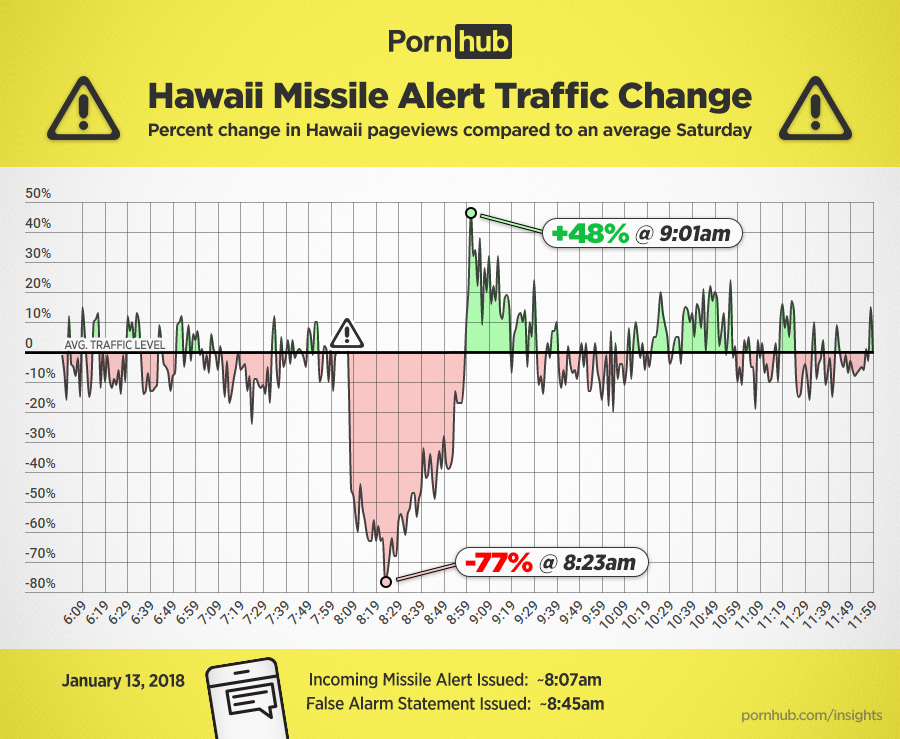
\includegraphics{C:/Users/the_l/Dropbox/00 Current teaching/dataScience/DataSciLibArts/images/pornHubHawaii.png}
\caption{pornHubHawaii}
\end{figure}

What is interesting here is not that PornHub traffic dropped during the
missile alert, but that it increased afterwards - as if the average
Hawaiian (and tourist) more or less made up for lost time afterwards.
(Data are pageviews compared to the previous two Saturdays).

\chapter{The ubiquity of data}\label{the-ubiquity-of-data}

\begin{figure}
\centering
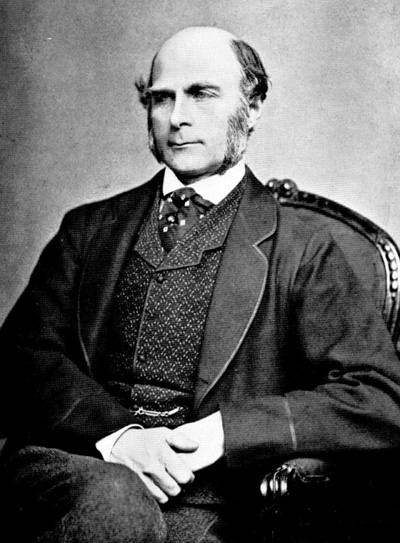
\includegraphics{C:/Users/the_l/Dropbox/00 Current teaching/dataScience/DataSciLibArts/images/Francis_Galton_1850s.jpg}
\caption{Francis\_Galton\_1850s}
\end{figure}

\section{IQ, whinnies and wines}\label{iq-whinnies-and-wines}

Empiricism is at the core of science. In psychology, the empirical
measurement of intelligence, vocational interest, and personality
transformed ideas about ``individual differences'' from speculation to
science.

Data Science is not new. A good beginning point is Sir Frances Galton
(above), who in the late 19th C is alleged to have declared ``whenever
you can, \emph{count}.'' At about the same time, the French psychologist
Alfred Binet sought to better identify schoolchildren with special needs
who would particularly benefit from smaller classes. His method was to
examine differences between children identified as better versus slower
learners on a wide range of tests which might be related to school
performance; he combined the successful ones to create the prototype for
the modern intelligence test.

As \citet{stephens2017everybody} recounts, Jeff Seder applies a similar
logic to examine the characteristics of horses associated with success.
Reminiscent of Binet's method, Seder finds enlarged left ventricle
associated with success. {[}but now that others know this, left
ventricle will not distinguish winners from losers.{]}

\emph{There it was, stark and clear, the reason that Seder and his team
had become so obsessed with No. 85. His left ventricle was in the
99.61st percentile! Not only that, but all his other important organs,
including the rest of his heart and spleen, were exceptionally large as
well. Generally speaking, when it comes to racing, Seder had found, the
bigger the left ventricle, the better. But a left ventricle as big as
this can be a sign of illness if the other organs are tiny. In American
Pharoah, all the key organs were bigger than average, and the left
ventricle was enormous. The data screamed that No. 85 was a 1-in-100,000
or even a one-in-a-million horse.} (p.~70-71).

This method has been referred to as ``brute force empiricism.'' The
question here is what works, not why. We may find it interesting to
speculate why Strawberry Pop-Tarts are particularly popular in
hurricanes (p.~71), but from the standpoint of Wal-Mart and its
customers, this is less important than stocking the shelves to satisfy
the demand that exists.

To predict the quality (as indexed by the price) of Bordeaux wines, a
regression equation works well:

Price = 12.145 + 0.00117 winter rainfall + 0.0614 average growing season
temperature -- 0.00386 harvest rainfall. (p.~73)

\section{The success of Google and the nature of
networks}\label{the-success-of-google-and-the-nature-of-networks}

Analyses of Google searches can reveal the flu and, perhaps, the
unemployment rate. (which is correlated with searches for porn sites and
solitaire). Google searches return an ordered list of sites based on a
modified Page Rank algorithm, which is a measure of network centrality.
Page Rank is what made Google better than early search engines such as
Alta Vista.

Google as a datasource
\citep[(\url{https://medium.com/}][]{pewresearch/using-google-trends-data-for-research-here-are-6-questions-to-ask-a7097f5fb526}()).
Includes Google Trends, Google Correlate, and Google books
(\url{https://books.google.com/ngrams}).

\begin{quote}
Google correlate (I tried this but it is finicky / weeks must begin on a
sunday - enter a time series, see what correlates with it.) \emph{Data
challenge: Find an interesting time series, use google correlate to find
something that it is associated with}
\end{quote}

\section{Words as data}\label{words-as-data}

Differences between liberals and conservatives, men and women, the old
and young, and extraverts and introverts can be informed by texts
ranging from the content of digitized books (Google Ngrams) to posts on
social media. Culturenomics (check spelling) can be revealing but is
challenging. Historians claim that the Civil War marked a transition
from thinking (or writing) about the US as a plural (\emph{The United
States are\ldots{}}) to a singular (\emph{The United States
is\ldots{}}). But analyses of the content of books in the Google Ngram
corpus revealed that the shift occurred a generation later.

There are two lessons here, the specific one about how the image of the
US changed more slowly than believed, the other, more general one is
that disciplines outside of the sciences are also increasingly informed
by the new empiricism. This is true not just for history but also for
literature; sentiment analysis can be applied to reveal the structure of
stories. (And analyses of Kindle data can reveal just where people stop
reading. I'm not sure if contemporary literature is auto-tuned to this,
but it is just a matter of time.)

\textbf{{[}note Gentzkow and Shapiro study of 2005 congressional
record{]}}

\section{Pictures as data}\label{pictures-as-data}

Scanned yearbooks from US High schools since 1905 show an increasing
number of smiles.

New approaches for measuring economic development include lights from
space, cell phone snaps at fruit stands.

\emph{These days, a data scientist must not limit herself to a narrow or
traditional view of data. These days, photographs of supermarket lines
are valuable data. The fullness of supermarket bins is data. The
ripeness of apples is data. Photos from outer space are data. The
curvature of lips is data. Everything is data!} (p.~104)

\chapter{\texorpdfstring{The `honesty' of
data}{The honesty of data}}\label{the-honesty-of-data}

In Chapter 4, \citet{stephens2017everybody} argues that making the
private public overcomes the limitations of traditional self-report
data.

\emph{People consistently gave wrong information, in ways that made them
look good. Fewer than 2 percent reported that they graduated with lower
than a 2.5 GPA. (In reality, about 11 percent did.) And 44 percent said
they had donated to the university in the past year. (In reality, about
28 percent did.)}

\textbf{There are two types of lying that are conflated - lying to
ourselves and lying to others.}

\emph{Lying to oneself may explain why so many people say they are above
average. How big is this problem? More than 40 percent of one company's
engineers said they are in the top 5 percent. More than 90 percent of
college professors say they do above-average work. One-quarter of high
school seniors think they are in the top 1 percent in their ability to
get along with other people.} (p.~107-108).

On the Internet\ldots{} are we more truthful? \emph{Google can display a
bias toward unseemly thoughts, thoughts people feel they can't discuss
with anyone else.} (p.~111).

Topics associated with shame and guilt are particularly likely to show a
difference between the private and the public.

\section{Sex}\label{sex-1}

\textbf{What percent of people are gay?} Surveys suggest differences
between states. But differences in searches for gay porn are far
smaller. Many men are in the closet, hiding even from their wives:
\emph{``Gay'' is 10 percent more likely to complete searches that begin
``Is my husband .~.~.'' than the second-place word, ``cheating.'' It is
eight times more common than ``an alcoholic'' and ten times more common
than ``depressed.'' Most tellingly perhaps, searches questioning a
husband's sexuality are far more prevalent in the least tolerant
regions. The states with the highest percentage of women asking this
question are South Carolina and Louisiana.} (p.~116-117).

\textbf{How often do people have sex?} \emph{On Google, there are
sixteen times more complaints about a spouse not wanting sex than about
a married partner not being willing to talk. There are five and a half
times more complaints about an unmarried partner not wanting sex than an
unmarried partner refusing to text back. And Google searches suggest a
surprising culprit for many of these sexless relationships. There are
twice as many complaints that a boyfriend won't have sex than that a
girlfriend won't have sex. By far, the number one search complaint about
a boyfriend is ``My boyfriend won't have sex with me.''} (p.~122-123)

\textbf{What are other people's sex lives like?} \emph{when men do look
for tips on how to give oral sex, they are frequently not looking for
ways of pleasing another person. Men make as many searches looking for
ways to perform oral sex on themselves as they do how to give a woman an
orgasm. (128)}

\section{Hate and prejudice}\label{hate-and-prejudice}

Stereotypes about other groups as evidenced by autocompletes for ``why
are {[}Black{]} people \ldots{}'' Do these lie in a two dimensional
space (competent-incompetent and warm-cold)?

Areas where Obama underperformed in 2008 and 2012, relative to Kerry 4
years before, are those where people search for n------ on Google (e.g.,
n---- jokes). Similarly, in the 2016 Republican Primary, In 2016,
support for Trump in the Republican Primary was predicted by searches
for n----. (From my standpoint, this was perhaps Stephens-Davidowitz
most important work). These searches outperformed, for example, the
performance of regions on the IAT.

\section{The internet and division}\label{the-internet-and-division}

People are more likely to encounter someone with different political
beliefs on the internet than in many other settings. This is partly
because we are likely to have more Facebook than real-world friends, and
the ``weak ties'' between different groups are especially important in
conveying information. (I hope that we'll return to this later when we
talk about networks).

\section{Child abuse and abortion}\label{child-abuse-and-abortion}

Searches re Child abuse (``my dad hit me) go up in recessions, but child
protective services get fewer calls.

\emph{In 2015, in the United States, there were more than 700,000 Google
searches looking into self-induced abortions\ldots{} there were some
4,000 searches looking for directions on coat hanger abortions,
including about 1,300 for the exact phrase ``how to do a coat hanger
abortion.'' There were also a few hundred looking into abortion through
bleaching one's uterus and punching one's stomach.}

\emph{Search rates for self-induced abortion were fairly steady from
2004 through 2007. They began to rise in late 2008, coinciding with the
financial crisis and the recession that followed. They took a big leap
in 2011, jumping 40 percent. The Guttmacher Institute, a reproductive
rights organization, singles out 2011 as the beginning of the country's
recent crackdown on abortion; ninety-two state provisions that restrict
access to abortion were enacted. Looking by comparison at Canada, which
has not seen a crackdown on reproductive rights, there was no comparable
increase in searches for self-induced abortions during this time. The
state with the highest rate of Google searches for self-induced
abortions is Mississippi, a state with roughly three million people and,
now, just one abortion clinic.} (p.~147-48)

\section{Be skeptical of the public self: Lesson from
Facebook}\label{be-skeptical-of-the-public-self-lesson-from-facebook}

Different sources of Big Data tell different stories, and are
susceptible to different biases. Twitter streams, for example, include
many bots, and weeding these out from humans can be challenging (and
will continue to be challenging as there is likely to be an arms race
between bots and algorithms for detecting them).

Google searches may be biased toward questions and topics we would be
unlikely to share with others, towards the darker aspects of
personality.

And Facebook data is, in some respects, just the opposite of this,
presenting an overly rosy picture of who we are. The notion that our
internet self is distorted is not new - the iconic Peter Steiner cartoon
below dates from 1993.

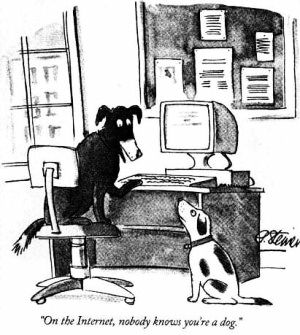
\includegraphics{C:/Users/the_l/Dropbox/00 Current teaching/dataScience/DataSciLibArts/images/Internet_dog.jpg}
d

\citet{stephens2017everybody} illustrates some of the ways in which our
social media selves are distorted - we read the \emph{Atlantic} rather
than the \emph{National Enquirer} for example. Facebook is, he writes
``\emph{digital brag-to-my-friends-about-how-good-my-life-is serum}''
(p.~152).

Spending time on social media is associated with depressed mood.

\section{Customers: Lessons from
Netflix}\label{customers-lessons-from-netflix}

Behavior is more telling than self report, and as a result, algorithms
may know us better than we know ourselves. Netflix no longer asks you to
create a queue of movies you would like to watch, because these
``aspirational'' choices correspond poorly with what we will in fact
watch.

\emph{Netflix learned a similar lesson early on in its life cycle: don't
trust what people tell you; trust what they do. Originally, the company
allowed users to create a queue of movies they wanted to watch in the
future but didn't have time for at the moment. This way, when they had
more time, Netflix could remind them of those movies. However, Netflix
noticed something odd in the data. Users were filling their queues with
plenty of movies. But days later, when they were reminded of the movies
on the queue, they rarely clicked. What was the problem? Ask users what
movies they plan to watch in a few days, and they will fill the queue
with aspirational, highbrow films, such as black-and-white World War II
documentaries or serious foreign films. A few days later, however, they
will want to watch the same movies they usually want to watch: lowbrow
comedies or romance films. People were consistently lying to themselves.
Faced with this disparity, Netflix stopped asking people to tell them
what they wanted to see in the future and started building a model based
on millions of clicks and views from similar customers. The company
began greeting its users with suggested lists of films based not on what
they claimed to like but on what the data said they were likely to view.
The result: customers visited Netflix more frequently and watched more
movies. ``The algorithms know you better than you know yourself,'' says
Xavier Amatriain, a former data scientist at Netflix.} (p.~156-157)

\section{Can we handle the truth?}\label{can-we-handle-the-truth}

Should we take this as good news or as bad?
\citet{stephens2017everybody} suggests that much of this can be
comforting - that seeing that others are insecure, are struggling with
their sexualities, or are concerned with the mundane rather than
profound. It can open our eyes to hidden problems of abuse, and, perhaps
most importantly, can point us towards interventions that can reduce
hatred.(But political language can be tailored to empirically divide us
rather than bring us together as well).

\chapter{Approaches to prediction}\label{approaches-to-prediction}

In Chapter 5, Stephens-Davidowitz examines what he calls the ``third
power of Big Data.'' That is, large data allows closer examination of
small subsets of humans (by looking at a large set of data for each of
them)

\section{Imprinting}\label{imprinting}

Why does one like a certain team - such as the Mets?
\citet{stephens2017everybody} presents evidence in support of an
\emph{imprinting hypothesis} - that there is a critical age.
Specifically, the Mets are very popular among those born in 1962 and in
1978 - and the Mets won the World Series in 1968 and 1986. This suggests
a critical age of 7 or 8.

He considers a study by Ghitza and Gelman, which finds some evidence for
a similar effect for politics - that the relevant age is between 14 and
24, at which point the popularity of the incumbent president will shape
political ideology for life.

What other things might show some imprinting effects, and how might this
be assessed?

\section{Regional effects and
contagion}\label{regional-effects-and-contagion}

Differences between countries in economic mobility are large, and the US
does badly, but there are pockets within the US in which this is less
true. Why?

For the wealthy, life expectancy is not highly related to where one
lives. For the poor, however, it is. \citet{stephens2017everybody}
argues that a good predictor of life expectancy among poor city-dwellers
is the ``number of rich people who live there.'' He argues that this is
due to contagion.

A more convincing contagion effect is seen in the study of IRS data.
People are likely to report self-reported income that maximizes their
tax refund; but this effect is highly localized, much more prevalent in
places like Miami (30\%) than Philadephia (2\%)\emph{.}

\emph{What predicts who is going to cheat? What is it about places that
have the greater number of cheaters and those that have lower numbers?
We can correlate rates of cheating with other city-level demographics
and it turns out that there are two strong predictors: a high
concentration of people in the area qualifying for the Earned Income Tax
Credit and a high concentration of tax professionals in the
neighborhood. What do these factors indicate? Chetty and the authors had
an explanation. The key motivator for cheating on your taxes in this
manner was information. Most self-employed one-kid taxpayers simply did
not know that the magic number for getting a big fat check from the
government was \$9,000. But living near others who might---either their
neighbors or tax assisters---dramatically increased the odds that they
would learn about it.} (p.~189-190).

\citet{stephens2017everybody} goes on to examine data such as Wikipedia
listings by geographical area, then between-country data on beliefs and
concerns about pregnancy.

He stratifies data by time, too, and finds that violence rates go
\emph{down,} not up, when violent movies appear. A closer examination of
the data revealed that this was particularly true when the young men who
were their audience were likely to be in the theater.

\section{Nearest neighbor analysis}\label{nearest-neighbor-analysis}

PECOTA and baseball doppelgangers.

This could, and will, make a difference in the prediciton of health
outcomes in the years to come.

\chapter{Experiments on us}\label{experiments-on-us}

In Chapter 6, \citet{stephens2017everybody} turns to the fourth power of
Big Data - rapid controlled experiments which tell us what works and
what does not.

\section{A/B testing}\label{ab-testing}

What color is the web, and why?

Obama campaign and choice of slogan.

\emph{The lesson of A/B testing, to a large degree, is to be wary of
general lessons. Clark Benson is the CEO of ranker.com, a news and
entertainment site that relies heavily on A/B testing to choose
headlines and site design. ``At the end of the day, you can't assume
anything,'' Benson says. ``Test literally everything.''} (p.~216-217)

The web you see on your phones and on your PCs is a web that is
experimentally designed to hold your attention as effectively and
powerfully as possible. You are not immune to this
\citep{alter2017irresistible}.

\section{Natural experiments}\label{natural-experiments}

The value of Super Bowl ads - although they cost millions, there is a
ROI of 2 or 3 to 1 : \emph{we looked at whether when a company
advertises a movie in the Super Bowl, they see a big jump in ticket
sales in the cities that had higher viewership for the game.} (p.~224)

When government or insurance companies change their compensation rates
for certain procedures, those procedures change in frequency. Patients
derive little if any added benefit from these.

\subsection{Do schools matter?}\label{do-schools-matter}

Effects of prestigious schools is less than it seems\ldots{}

``Elite Illusion.'' The effects of Stuyvesant High School? Nil. Nada.
Zero. Bupkus. Students on either side of the cutoff ended up with
indistinguishable AP scores and indistinguishable SAT scores and
attended indistinguishably prestigious universities. The entire reason
that Stuy students achieve more in life than non-Stuy students, the
researchers concluded, is that better students attend Stuyvesant in the
first place. Stuy does not cause you to perform better on AP tests, do
better on your SATs, or end up at a better college.* (p.~236)

But my analysis of Psych licensing scores.

\chapter{Limits of Big data}\label{limits-of-big-data}

Remaining chapters of \citet{stephens2017everybody}

Begins with a discussion of Larry Summers. Mentions the differential
variability hypothesis (see also Dangerous idea paper). Then moves on to
the question of whether Big Data can predict the stock market - the
answer is no.

\section{The curse of dimensionality}\label{the-curse-of-dimensionality}

With many predictors, some will appear effective by chance. This infects
the search for causal and robust relationships, both in scientific
hypothesis testing and in everyday life.

\section{The overemphasis on the
measurable}\label{the-overemphasis-on-the-measurable}

Not just pedometers, but baseball offense as opposed to defense, and
ways of thinking in which there are right as opposed to insightful and
creative answers. In school, the emphasis on speed rather than
thoughfulness.

\section{Ethical concerns}\label{ethical-concerns}

\emph{Do corporations have the right to judge our fitness for their
services based on abstract but statistically predictive criteria not
directly related to those services?} (p.~261)

Casinos know that (problem) gamblers have pain points, points at which
their losses will be so large that they will be unlikely to come back to
the casino. Casinos will be successful if they can stop gamblers from
getting to (rather beyond) this point.

\emph{Scott Gnau, general manager of Terabyte, explains, in the
excellent book Super Crunchers, what casino managers do when they see a
regular customer nearing their pain point: ``They come out and say, `I
see you're having a rough day. I know you like our steakhouse. Here, I'd
like you to take your wife to dinner on us right now.'\,''} (p.~264)

With more data, more companies will price discriminate, charging not
just what the market will bear, but what they can get from us, based
upon analysis of `doppelgangers' or nearest neighbors\ldots{}

\section{Individual versus group level
predictions}\label{individual-versus-group-level-predictions}

At an individual level, search data may be effectively useless.

\section{Conclusion: Data and
science}\label{conclusion-data-and-science}

\emph{Frankly, the overwhelming majority of academics have ignored the
data explosion caused by the digital age. The world's most famous sex
researchers stick with the tried and true\ldots{}for every idea I have
talked about in this book, there are a hundred ideas just as important
ready to be tackled.}

\emph{For any disease, we can explore Google search data or other
digital health data\ldots{}we can find if there are any tiny pockets of
the world where prevalence of this disease is unusually high or
unusually low.}

\emph{We might call this---taking a simple method and utilizing Big Data
to perform an analysis several hundred times in a short period of
time---science at scale.}

\emph{A/B testing can be used to uncover things more fundamental---and
socially valuable---than an arrow that gets people to click on an ad.
Benjamin F. Jones \ldots{} has helped create a platform, EDU STAR, which
allows for schools to randomly test different lesson plans. \ldots{}
students log in to a computer and are randomly exposed to different
lesson plans. Then they take short tests to see how well they learned
the material. Schools, in other words, learn what software works best
for helping students grasp material.} (p.~274-276).

\part{Part II Towards data
literacy}\label{part-part-ii-towards-data-literacy}

(Hal Varian - webcast next Wednesday at 3 PM)

\chapter{Principles of data
visualization}\label{principles-of-data-visualization}

\section{Opening thoughts}\label{opening-thoughts}

Graphs aren't just to inform, but to make you reflect.

We are concerned not just with the design of graphs, but with our role
in society as leaders, as arbiters of facts, as educators. We want to
foster data literacy.

How do people understand graphs? (NY Times series for schools).

How can you use graphs to tell people the truth in a way that they
understand?

When you see a graph, what do you notice, what do you wonder, and what
is the story? Is ``story telling'' what visualizations should be about?

A graph might begin with perception and understanding (the consumer),
with knowledge and design values (the producer), but it also reflects
the truth of the data. How much is each?

\section{Some early graphs}\label{some-early-graphs}

Visual displays of information reach back to prehistoric times; modern
graphs date back, arguably, to Playfair's 1786 \emph{Political Atlas} -
in which

*``\ldots{} spatial dimensions were used to represent nonspatial,
quantitative, idiographic, empirical data. Although it now seems natural
to represent, for example, rising and falling imports over time as a
rising and falling line, it does not seem to have been done before that
time and was quite an accomplishment. Notably, in addition to the
statistical line chart, Playfair at one fell swoop single-handedly
invented most of the remaining forms of the statistical graphic
repertoire used today-the bar chart and histogram, the surface chart,
and the circle diagram or''pie chart.``*

\begin{figure}
\centering
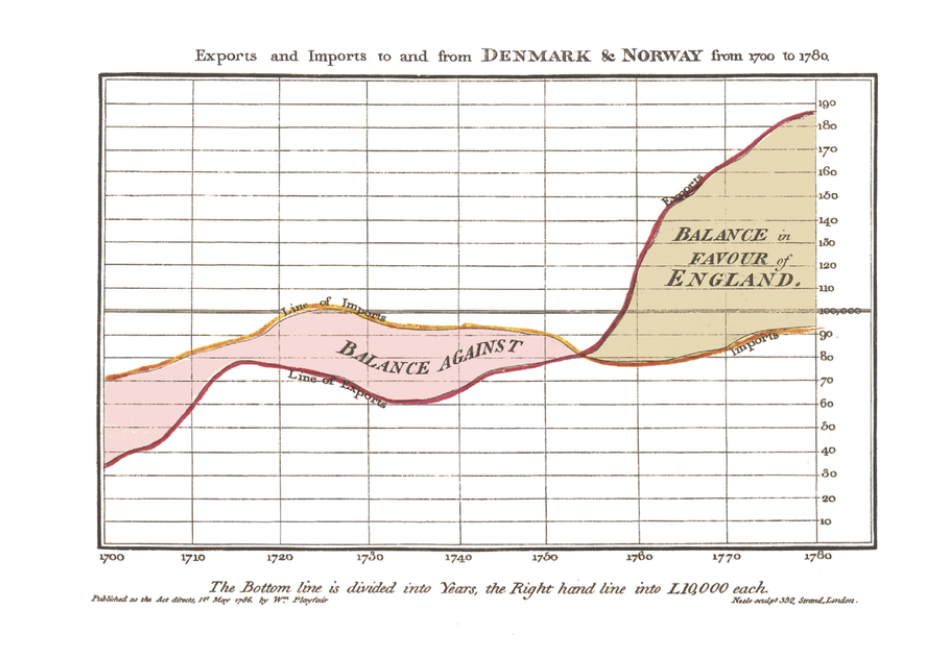
\includegraphics{C:/Users/the_l/Dropbox/00 Current teaching/dataScience/DataSciLibArts/images/playfair1786.png}
\caption{playfair1786}
\end{figure}

\href{https://robots.thoughtbot.com/analyzing-minards-visualization-of-napoleons-1812-march}{source}

\begin{center}\rule{0.5\linewidth}{\linethickness}\end{center}

\begin{enumerate}
\def\labelenumi{\arabic{enumi})}
\setcounter{enumi}{1}
\tightlist
\item
  The most important early graph is that of Minard. In class, we
  listened to the 1812 Overture while discussing this. Here's some
  background:
\end{enumerate}

``*Czar Alexander of Russia sees that Napoleon was becoming too
powerful, so he refuses to participate in this embargo. Angry at Czar
Alexander's decision, Napoleon gathers a massive army of over 400,000 to
attack Russia in June of 1812. While Russia's troops are not as numerous
as France's, Russia has a plan. Russian troops keep retreating as
Napoleon's troops move forward, burning everything they pass, ensuring
that the French forces could not take anything from their environment.
Eventually the French army follows the Russian army all the way to
Moscow during October, suffering major losses from lack of food. By the
time Napoleon gets to Moscow, he knows he has to retreat. As winter
settles into Europe and the temperature drops, Napoleon's troops suffer
even more losses, returning to France from lack of food, disease, and
weather conditions.``*

(The battle of Borodino, immortalized in Tolstoy's War and Peace, occurs
just before Moscow; the French army loses about 30000 men. Five cannon
shots in the overture mark this. And when Napoleon gets to Moscow, he
finds that the Russians had razed it before hand, so that there was
nothing there for them. Eleven more cannon here.)

\begin{figure}
\centering
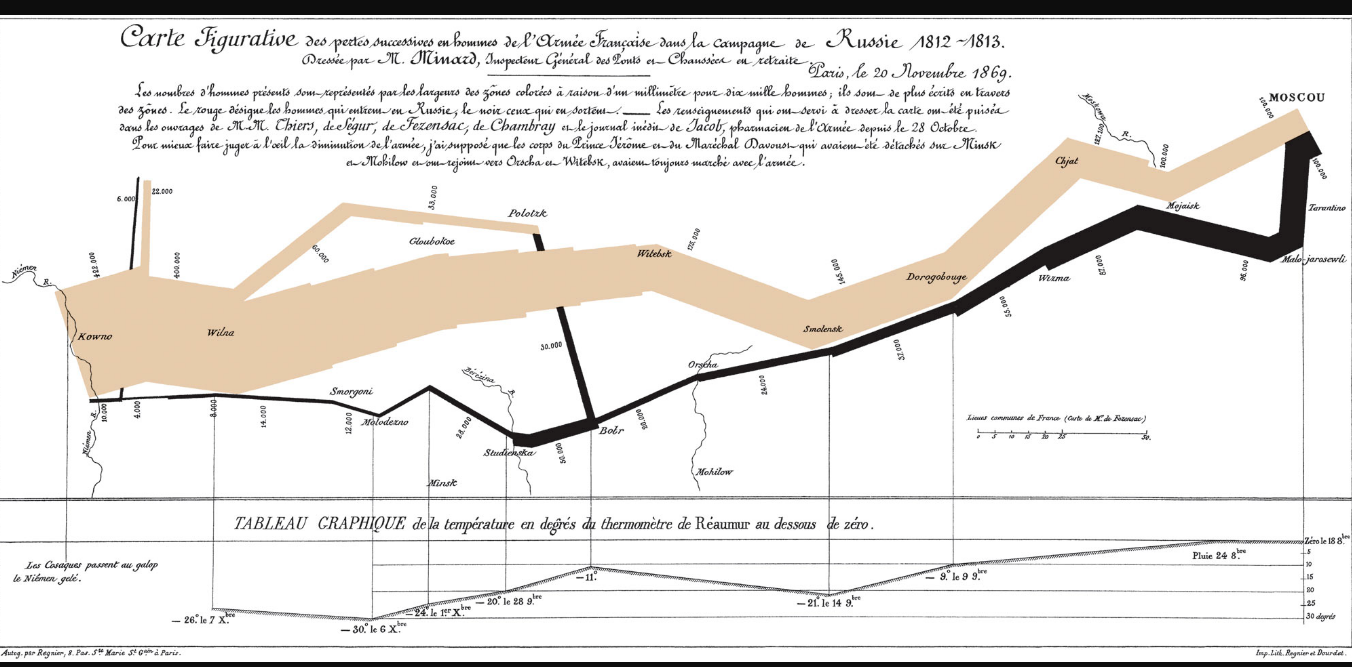
\includegraphics{C:/Users/the_l/Dropbox/00 Current teaching/dataScience/DataSciLibArts/images/minard1812.png}
\caption{minard1812}
\end{figure}

\href{https://datavizblog.com/2013/05/30/dataviz-history-charles-minards-flow-map-of-napoleons-russian-campaign-of-1812-polotsk-smolensk-and-on-to-borodino/}{source}

\begin{center}\rule{0.5\linewidth}{\linethickness}\end{center}

\section{Tukey's contributions}\label{tukeys-contributions}

Tukey and Exploratory Data Analysis (EDA). Begins with Tukey 1962
``Future of Data Analysis,'' continues with his ultimate publication of
EDA in 1977.

Tukey decries tallies (prone to error), and shows \textbf{stem and leaf
displays}, then box plots. He argues for transforming data to linearity
to uncover meaningful relationships, then to examine residuals to look
more closely.

\section{Approaches to graphs}\label{approaches-to-graphs}

A graph might begin with perception and understanding (the consumer),
with knowledge and design values (the producer), but it also reflects
the truth of the data. How much is each?

In thinking about how to design graphs, we can begin with abstract
theory, with principles of design informed by our understanding of
perception, or with empirical analyses of understanding and memory.

\section{Tufte: First principles}\label{tufte-first-principles}

\citet{tufte2001visual} describes \textbf{Graphical Excellence}. Graphs
should, among other things, ``Induce the viewer to think about the
substance, rather than about methodology, graphic design, the technology
of graphic productions, or something else.'' Graphs should ``Present
many numbers in a small space, make large data sets coherent, and
encourage the eye to compare different pieces of data.'' Graphs should
``serve a reasonably clear purpose: description, exploration,
tabulation, or decoration {[}and{]} be closely integrated with the
statistical and verbal descriptions of a data set.''"

Tufte concludes with the following Principles of Graphical Excellence,
which I quote verbatim: \textbf{\emph{Graphical excellence is the
well-designed presentation of interesting data---a}}
\textbf{\emph{matter of substance, of statistics, and of design.}}
\textbf{\emph{Graphical excellence consists of complex ideas
communicated with clarity,}} \textbf{\emph{precision and efficiency.}}
\textbf{\emph{Graphical excellence is that which gives to the viewer the
greatest number of}} \textbf{\emph{ideas in the shortest time with the
least ink in the smallest space.}} \textbf{\emph{Graphical excellence is
nearly always multivariate.}} \textbf{\emph{And graphical excellence
requires telling the truth.}}

\begin{figure}
\centering
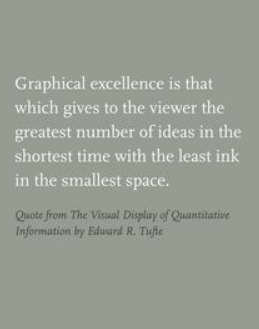
\includegraphics{C:/Users/the_l/Dropbox/00 Current teaching/dataScience/DataSciLibArts/images/tuftequote.png}
\caption{tuftequote}
\end{figure}

\begin{center}\rule{0.5\linewidth}{\linethickness}\end{center}

\subsection{An illustration of the cost of bad graphs: The Challenger
disaster}\label{an-illustration-of-the-cost-of-bad-graphs-the-challenger-disaster}

\begin{figure}
\centering
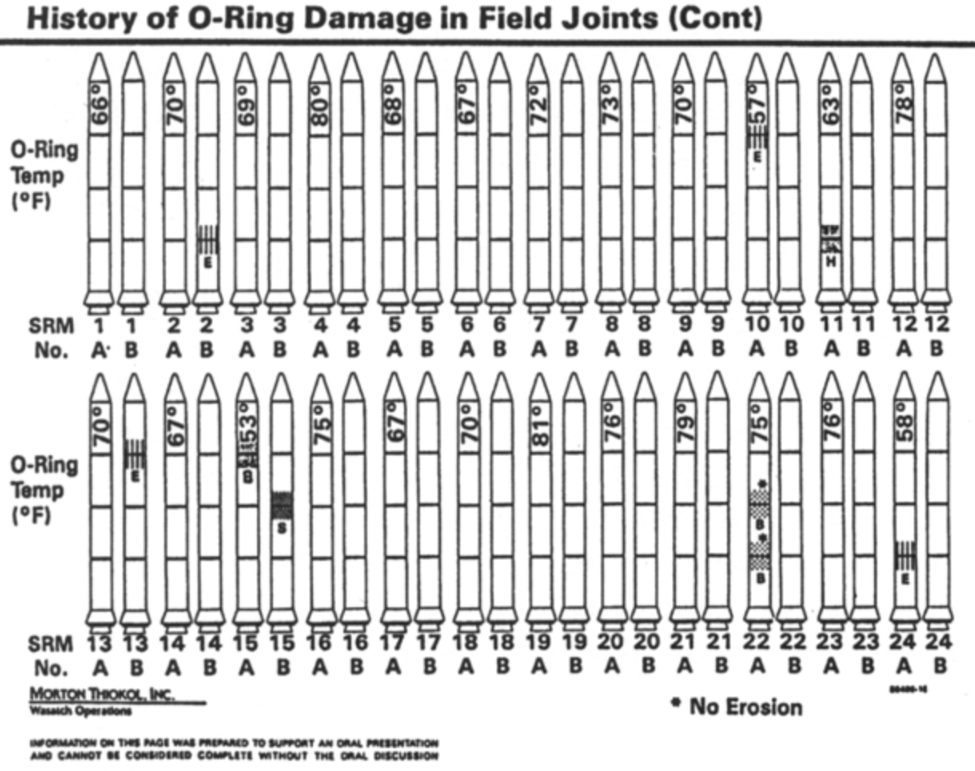
\includegraphics{C:/Users/the_l/Dropbox/00 Current teaching/dataScience/DataSciLibArts/images/mortonthiokolChallenger.png}
\caption{tufteChallenger}
\end{figure}

\begin{center}\rule{0.5\linewidth}{\linethickness}\end{center}

\begin{figure}
\centering
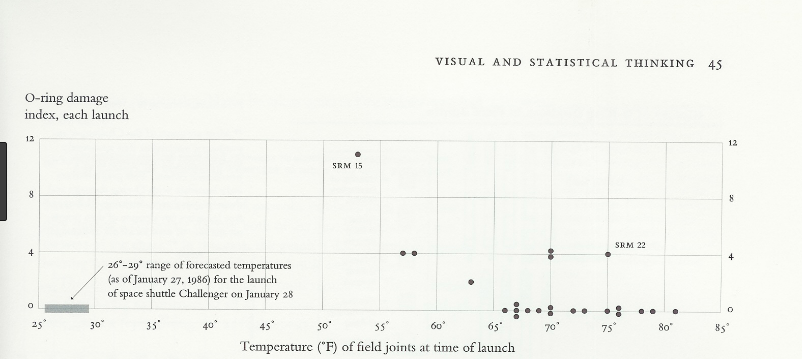
\includegraphics{C:/Users/the_l/Dropbox/00 Current teaching/dataScience/DataSciLibArts/images/tufteChallenger.png}
\caption{tufteChallenger}
\end{figure}

\begin{center}\rule{0.5\linewidth}{\linethickness}\end{center}

\section{Should graphs begin with psychological
theory?}\label{should-graphs-begin-with-psychological-theory}

\citet{wainer1981graphical} used Chernoff's faces to represent
multivariate data. Grounded in a psychological premise. Did they
succeed? Why or why not?

\begin{figure}
\centering
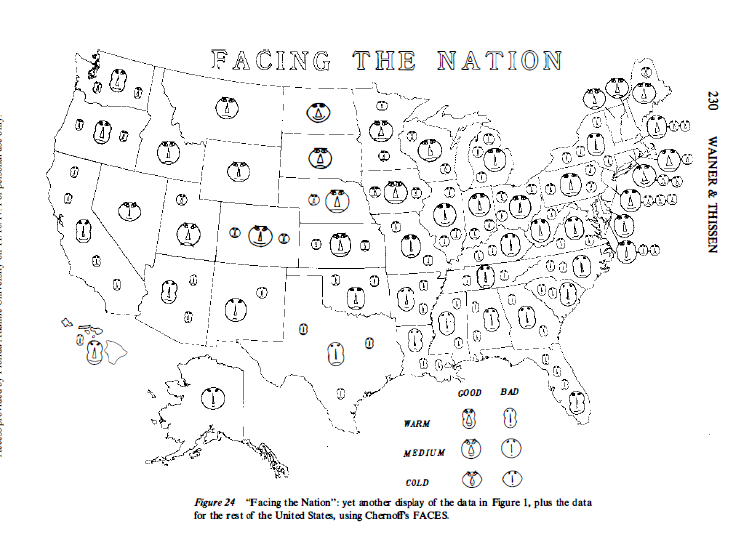
\includegraphics{C:/Users/the_l/Dropbox/00 Current teaching/dataScience/DataSciLibArts/images/Chernoff.png}
\caption{tufteChallenger}
\end{figure}

Population - the (log) number of faces/state

Literacy rate - size of the eyes (bigger = higher).

\% HS graduates - slant of the eyes (the more slanted = higher).

Life expectancy - the length of the mouth (the longer = longer).

Homicide rate - the width of the nose (the wider the nose the lower).

Income - the curvature of the mouth (the bigger the smile the higher the
income).

Temperature - the shape of the face (peanut= warmer, football= colder)

Longitude and latitude - The X and Y position of the face on the
coordinate axes of the paper represent the position of the state

\section{Further reading and
resources}\label{further-reading-and-resources}

This is only the beginning of a discussion of data visualizations.
\citet{healy2018viz} presents a more expanded discussion of this
treatment. He addresses the limitations of infographics, in which the
design purveys style over substance (this is what we may do in designing
presentations as well), and includes a rationale for a grammar of
graphics, as instantiated in the ggplot package in R that we will be
working with \citep{wickham2016r}. \citet{cleveland1985graphical}
examines graphs from a more rigorous psychological and empirical
viewpoint. The \href{http://datastori.es/}{Data Stories podcasts} are
often excellent, despite the challenge of an auditory medium for visual
displays. And your classmates on the Slack \#dataviz channel have things
to say as well.

\chapter{Statistics: Probability and
inference}\label{statistics-probability-and-inference}

In our first meeting on this, we discussed \citet{wainer2007most}. He
argues that deMoivre's equation is the most dangerous - this equation
(for the standard error) shows that variability decreases with the
square root of sample size. Other nominees include the linear regression
equation (and, in particular, how coefficients may change or reverse
when new variables are added) and regression to the mean. Regarding
linear regression, we discussed (a little) Simpson's paradox, that is,
that the direction of regression coefficients may change when additional
variables are added.

I argued that, from the standpoint of psychology, ignorance of
regression to the mean was arguably more `dangerous' than ignorance
about the central limit theorem and standard error, in particular
because regression effects contribute to an overestimate of the
effectiveness of punishment and an under-appreciation of the
effectiveness of positive reinforcement as tools for behavior change
\citep{hastie2010rational}.

We talked also about \citet{anscombe1973graphs} and his quartet, and how
visualizing data is valuable.

\section{More on probability}\label{more-on-probability}

Discrete probability is used to understand the likelihood of categorical
events. We can think of initial estimates of probability as subjective
or personal. For some events (\emph{what is the probability this plane
will crash?}), an estimate of probability can be drawn from a base rate
or relative frequency (e.g., \emph{p(this plane will crash) = (number of
flights with crashes/ number of flights)}). For other events (what is
the probability that the US President will resign or be impeached before
completing his term of office?), it may be hard to arrive at a suitable
base rate. Here, a number of subjective beliefs or principles may be
combined to arrive at a subjective or personal probability. In a sense,
all probability estimates begin with a personal belief such as this, in
part because the choice of the most informative base rate is often not
self-evident - in the former example, maybe we should consider a
reference group rates such as `for this airline' etc.
\citep[(][]{lanning1987some}. The personal origins of probability
estimates should become less important as we are exposed to data and
revise our estimates in accordance with Bayes theorem. But over the last
45 years, a substantial body of evidence has demonstrates that, under at
least some circumstances, we don't make estimates of probability in this
way.

There is a nice r markdown document discussing basic laws of probability
at Harvard's datasciencelabs repository:
\url{https://github.com/datasciencelabs/2017/blob/master/lectures/prob/discrete-probability.Rmd}.

We can also use probability with continuous variables such as systolic
blood pressure (that's the first one), which has a mean of approximately
120 and a standard deviation of 15. Continuous probability distributions
are handy tools for thinking about the meaning of scores, particularly
when we express scores in standard deviations from the mean (z scores).
More to the point, this way of thinking about probability is widely used
in questions of scientific inference, as, for example, in testing
hypotheses such that ``the average systolic blood pressure among a group
of people studying at Crux (hence caffeinated) will be significantly
greater than that of the population as a whole.''

This is the logic of \textbf{Null Hypothesis Significance Testing
(NHST)} - if the result in my Crux sample is sufficiently high, then I
say that I have rejected the null hypothesis, and found data which
support the hypothesis of interest.

\subparagraph{\texorpdfstring{\emph{Let's write up a sample study,
describing the methods we would use to test
this.}}{Let's write up a sample study, describing the methods we would use to test this.}}\label{lets-write-up-a-sample-study-describing-the-methods-we-would-use-to-test-this.}

\chapter{Reproducibility and the replication
crisis}\label{reproducibility-and-the-replication-crisis}

Probability theory is elegant, and the logic of NHST is compelling. But
philosophers of science have long recognized that this is not how
science works \citep{lakatos1969falsification}. (Consider, for example,
a simple test of whether gravity exists).

In recent years, the tension between \textbf{the false ideal of NHST}
and the real world of science has become increasingly evident. Within
psychology, experimental studies have often - even typically - failed to
replicate \citep{open2015estimating}. It's not just psychology
\citep{baker2016reproducibility}. One of the first important papers to
shine light in the area \citep{ioannidis2005most} came from medicine; it
suggested six contributing factors, which I quote verbatim here:

\emph{The smaller the studies conducted in a scientific field, the less
likely the research findings are to be true.}

\begin{itemize}
\tightlist
\item
  This stems directly from our discussion of the central limit theorem
  and the instability of results from small samples.
\end{itemize}

\emph{The smaller the effect sizes in a scientific field, the less
likely the research findings are to be true}

\begin{itemize}
\tightlist
\item
  We'll talk about effect size below.
\end{itemize}

\emph{The greater the number and the lesser the selection of tested
relationships in a scientific field, the less likely the research
findings are to be true.} (and) \emph{The greater the flexibility in
designs, definitions, outcomes, and analytical modes in a scientific
field, the less likely the research findings are to be true.}

\begin{itemize}
\tightlist
\item
  The ``problem'' of analytic flexibility leads to `p-hacking'
\end{itemize}

\emph{The greater the financial and other interests and prejudices in a
scientific field, the less likely the research findings are to be true}
and \emph{The hotter a scientific field (with more scientific teams
involved), the less likely the research findings are to be true.}

\begin{itemize}
\tightlist
\item
  Positive findings rise, and negative ones are ignored. And scientists
  are human, and subject to incentives.
\end{itemize}

Here's a video which provides some more context for the crisis:
\url{https://www.youtube.com/watch?v=42QuXLucH3Q} (12 mins)

\subsection{Answers to the reproducibility crisis I: On
NHST}\label{answers-to-the-reproducibility-crisis-i-on-nhst}

The first cluster of responses addresses problems with Null Hypothesis
Significance Testing (NHST). These include (a) justifying one's alpha -
making it more stringent, for example, for counter-intuitive claims
\citep{grange2018justify}, (b) changing the default p value from .05 to
.005 \citep{benjamin2017redefine}, and (c) abandon significance testing
altogether \citep{mcshane2017abandon}.

\citet{szucs2017null} goes into some of these issues in more detail and
discusses other limitations of significance testing, including the
dichotomous, all-or-none silliness of the accept/reject decision. (If
you play the NHST game, there is no `almost' significant, `approached
significance,' etc.).

\citet{leek2015statistics} argue that the problems are not merely with
NHST, but with the whole of data analysis. They maintain that better
training in data science - courses like ours, perhaps, are part of the
answer.

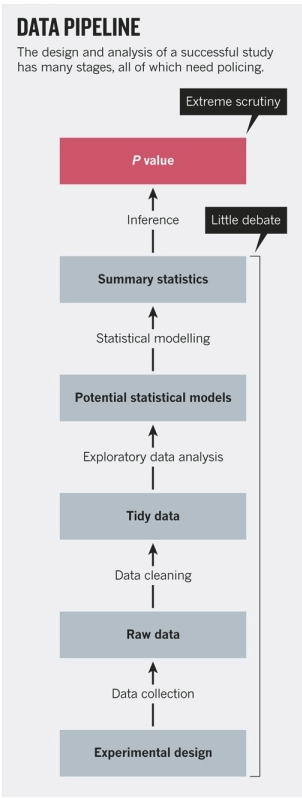
\includegraphics{C:/Users/the_l/Dropbox/00 Current teaching/DataScience/DataSciLibArts/images/leek2015pipeline.PNG}
(figure)

\subparagraph{\texorpdfstring{\citet{munafo2017manifesto} also argue
that threats to reproducible science occur at a number of places in
science, not just with the evaluation of
hypotheses.}{@munafo2017manifesto also argue that threats to reproducible science occur at a number of places in science, not just with the evaluation of hypotheses.}}\label{munafo2017manifesto-also-argue-that-threats-to-reproducible-science-occur-at-a-number-of-places-in-science-not-just-with-the-evaluation-of-hypotheses.}

\begin{figure}
\centering
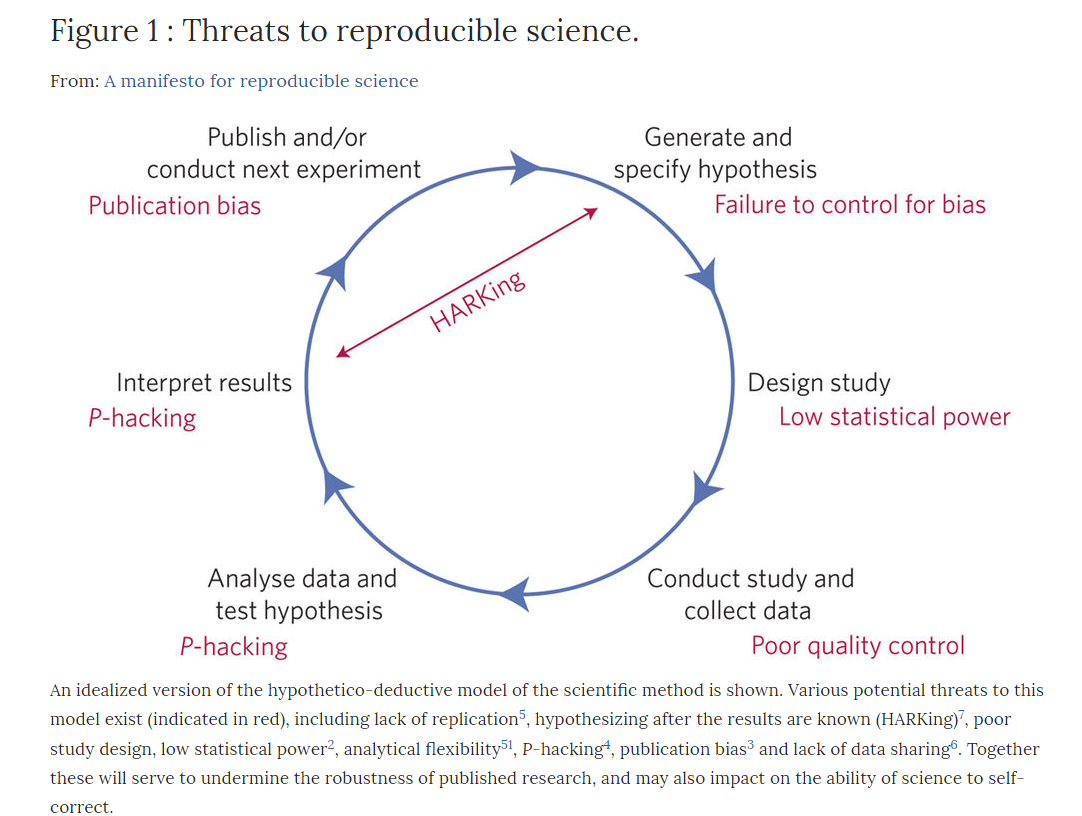
\includegraphics{C:/Users/the_l/Dropbox/00 Current teaching/DataScience/DataSciLibArts/images/munarothreats.PNG}
\caption{munarothreats}
\end{figure}

\subsection{Answers to the reproducibility crisis II:
Pre-registration}\label{answers-to-the-reproducibility-crisis-ii-pre-registration}

The second type of response includes (d) preregistering your work
\citep{miguel2014promoting}. There's a video here:
\url{https://www.futurelearn.com/courses/open-social-science-research/0/steps/31436}
(5 mins). For randomized controlled trials, consider
socialscienceregistry.org, and for more general use, use the open
science framework page. Incidentally, you can post your theses after
they are finished at \url{https://thesiscommons.org}.

garden of the forking paths

There's a collection of papers here\ldots{}
\url{https://www.nature.com/collections/prbfkwmwvz/}

Showing exactly what you have done and how (and why) you got there is at
the core of reproducible science.

\subparagraph{\texorpdfstring{\emph{What would results for our sample
study look like? How many of these problems would it face? What should
we do about
it?}}{What would results for our sample study look like? How many of these problems would it face? What should we do about it?}}\label{what-would-results-for-our-sample-study-look-like-how-many-of-these-problems-would-it-face-what-should-we-do-about-it}

\part{Part III Towards data
proficiency}\label{part-part-iii-towards-data-proficiency}

In this part of the class we will get into the nuts and bolts of R.

\chapter{Literate programming with R
markdown}\label{literate-programming-with-r-markdown}

A note from chapter 4 (coding basics): use assignment (x \textless{} -
3+4) rather than x = 3 + 4 because it is more clear.

Showing your work - for you as well as others - is another part of
reproducible science. R Markdown documents allow you to include
comments, scripts, and results in a single place.

We begin R4DS 6 (\emph{Workflow: Scripts}, p.~110) which shows the R
studio interface and encourages you to save your work using
\emph{scripts}.

You will save your work in \emph{projects} - which isolate your work,
setup files, etc., into different directories. (See r4ds, chapter 8). To
reinforce the idea that your unit of analysis in R is ``the project''
rather than ``the script'', consider associating your Rmd filetype with
your markdown editor, and only your Rproj filetype with R studio.

The R markdown language is discussed in R4ds, Chapter 27 (p.~505).

\section{A challenge}\label{a-challenge-1}

Working with two of your classmates, write an R markdown document titled
``The most dangerous equation?'' which (a) in the introduction,
discusses \citet{wainer2007most}, (b) then illustrates regression to the
mean and (c) deMoivre's equation, ideally (d) using the examples of
`punishment' and `sex differences in variability' discussed in class and
the text, respectively.

Prepare a presentation using Rpres which summarizes your argument and
findings. Present this in class on 2/26.

(One starting point: the aforementioned r markdown document discussing
basic laws of probability at Harvard's datasciencelabs repository:
\url{https://github.com/datasciencelabs/2017/blob/master/lectures/prob/discrete-probability.Rmd}.

\section{r markdown}\label{r-markdown}

Goals and functions

\begin{itemize}
\tightlist
\item
  one goal is making your work clear to others, and to a later you
\end{itemize}

Parts

\begin{itemize}
\tightlist
\item
  YAML header: Some output formats
\item
  Text formatted in markdown
\item
  R code (chunks) surrounded by code fences
\item
  (occasionally, inline code)
\end{itemize}

See \textbf{Rmd cheatsheet (on Slack)}

\section{univariate data}\label{univariate-data}

kable and other approaches to generating output

exercise 27.4.7 2
(\url{https://raw.githubusercontent.com/hadley/r4ds/master/rmarkdown/diamond-sizes.Rmd})

(make a report)

\chapter{ggplot2}\label{ggplot2}

\section{r dialects}\label{r-dialects}

Several approaches to graphics (and everything else!) in r; see
\textbf{syntax cheatsheet} (on Slack)

\section{logic of ggplot}\label{logic-of-ggplot}

\subsection{\texorpdfstring{the \textbf{data visualization cheatsheet}
(on
Slack)}{the data visualization cheatsheet (on Slack)}}\label{the-data-visualization-cheatsheet-on-slack}

a layered system of graphics. goal is to come up with some rules for
good graphs, and a syntax with which to understand it

\section{playing with ggplot2}\label{playing-with-ggplot2}

play along with Chapter 3

get ggplot2 to work

exercises 3.2.4 (what do you see?)

exercises 3.3.1 (a little further)

\section{playing with new data}\label{playing-with-new-data}

get data - sources include \url{https://github.com/idc9/stor390} and
online data sets in R

pull out no more than five variables from the dataset

\subsection{3.4 multivariate data}\label{multivariate-data}

exercises 3.5.1

\chapter{References}\label{references}

\bibliography{../dataSciRefs.bib}


\end{document}
